%\documentclass[japanese]{jssst_ppl} %%
 \documentclass[english]{jssst_ppl} %% English
% \documentclass[japanese,draft]{jssst_ppl} %% You can use the draft option
\usepackage{amsmath,amsthm,amssymb,amsfonts,extarrows,geometry,amsopn,enumerate}
\usepackage{graphicx}
\usepackage{boxedminipage}
\usepackage{url}

% set some new commands %
\newcommand\tB{\;|\;}
\newcommand\LET{\mathbf{let}\;}
\newcommand\FREE{\mathbf{free(x)}\;}
\newcommand\IN{\mathbf{in}\;}
\newcommand\SKIP{\mathbf{skip}}
\newcommand\Rtab{\; \; \; \;}
\newcommand\NULL{\mathbf{null}\;}
\newcommand\IFNULL{\mathbf{ifnull}\;}
\newcommand\THEN{\mathbf{then}\;}
\newcommand\ELSE{\mathbf{else}\;}
\newcommand\Lcc{\left(}
\newcommand\Rcc{\right)}
\newcommand\Lfc{\left\{}
\newcommand\Rfc{\right\}}
\newcommand\Lb{\left[}
\newcommand\Rb{\right]}
\newcommand\coma{,\;}
\newcommand\MALLOC{\mathbf{malloc()}\;}
\newcommand\Malloc{\mathbf{malloc}}
\newcommand\Free{\mathbf{free}}
\newcommand\Cirx{(x)}
\newcommand\dtb{\;\;\ \;\;\ \;\;\ \;\;\  }
\newtheorem{theorem}{Theorem}[section]
\newtheorem{lemma}[theorem]{Lemma}
\newtheorem{proposition}[theorem]{Proposition}
\newtheorem{corollary}[theorem]{Corollary}
\newtheorem{myDef}{Definition}

\theoremstyle{definition}
\newtheorem{exmp}{Example}[section]

\newenvironment{nospaceflalign*}
 {\setlength{\abovedisplayskip}{0pt}\setlength{\belowdisplayskip}{0pt}%
  \csname flalign*\endcsname}
 {\csname endflalign*\endcsname\ignorespacesafterend}

\newcommand\todo[1]{{\bf KS: {#1}}}

\title{A Behavioral Type System for \\ Memory-Leak Freedom}
\author{Qi Tan, Kohei Suenaga, Atsushi Igarashi}
\inst{
    Department of Communications and Computer Engineering\\
    Graduate School of Informatics\\
    Kyoto University\\
\texttt{\{tanki,ksuenaga,igarashi\}@fos.kuis.kyoto-u.ac.jp}
%\medskip\par%
}
\begin{document}
\maketitle
\begin{abstract}
We propose a type system to abstract the behavior of a program under manual memory management. Our type system uses CCS-like processes as types where each action corresponds to an allocation and a deallocation of a fixed-size memory block. The abstraction obtained by our type system makes it possible to estimate an upper bound of memory consumption of a program. Hence, by using our type system with another safe-memory-deallocation analysis proposed by Suenaga and Kobayashi, we can verify memory-leak freedom even for nonterminating programs.  We define the type system, prove type soundness, and show a type reconstruction procedure that estimates an upper bound of memory consumption using an off-the-shelf model checker.
\end{abstract}

\section{Introduction}
\subsection{Motivation and Problems}
Manual memory management primitives (e.g., \texttt{malloc} and \texttt{free} in C) often cause that forgetting to deallocate memory cells after use, which we call \emph{memory leaks}. It can diminish the performance of the computer by reducing the amount of available memory cells. Memory leaks may not be serious or even detectable by normal means. Normal memory used by an application is released when application terminates. This means that a memory leak in a program that only runs for a short time may not be noticed and is rarely serious. However, in the real-world programs, nonterminating programs such as Web servers and operating systems are very important. If memory leaks in such nonterminating programs, eventually, too much of the available memory cells may become allocated and all or part of the system stops working correctly~\cite{wiki:xxx}.

\begin{exmp}\label{ex:ex1}
Functions $h$ and $h'$ shown in Figure~\ref{ex:np} describe memory-leak freedom and memory leaks in nonterminating programs. Function $h$ requires two memory cells at most, whereas function $h'$ requires unbounded number of memory cells to be executed.
\begin{figure}[h]
1  \Rtab $h(x)$= \dtb \dtb\dtb\Rtab$h'(x)$= \\
2  \dtb $\LET \; x = \MALLOC  \; \IN$ \dtb \Rtab$\LET \; x = \MALLOC  \; \IN$\\
3  \dtb $\LET \; y = \MALLOC  \; \IN$ \dtb \Rtab$\LET \; y = \MALLOC  \; \IN$\\
4  \dtb $\Free(x)$; $\Free(y) $;\;$h(x)$ \dtb \Rtab$h'(x)$; $\Free\Cirx$; \ $\Free(y)$
\caption{memory leaks in nonterminating programs.}
\label{ex:np}
\end{figure}
\end{exmp}

Most of the static analysis of memory-leak freedom proposed so far~\cite{DBLP:conf/aplas/SuenagaK09, DBLP:conf/sas/OrlovichR06,DBLP:conf/pldi/HeineL03,DBLP:conf/sigsoft/XieA05,DBLP:journals/scp/SwamyHMGJ06} deal with only \emph{partial memory-leak freedom}: if a program terminates, allocated memory cells are all deallocated at the end. For example, the type system by Suenaga and Kobayashi~\cite{DBLP:conf/aplas/SuenagaK09}, which is called \textbf{SK} type system in our paper, guarantees that (1) a well-typed program does not conduct illegal accesses and that (2) after execution of a well-typed program, all the memory cells are deallocated.

We tackle the problem of verifying \emph{total memory-leak freedom} in this paper.\footnote{we often write memory-leak freedom for \emph{total} memory-leak freedom.} By a program being totally memory-leak free, we mean that the program requires only a bounded amount of memory even if it does not terminate.

\subsection{Approach}
From examples in Figure~\ref{ex:np}, we notice that a simple way to guarantee memory-leak freedom for nonterminating programs is to check whether the number of allocations and deallocations is balanced before recursive call. If balanced, the program consumes bounded number of memory cells, say function $h$ allocates two memory cells and deallocates them before recursive call, it consumes two memory cells at most once; if not balanced, as function $h'$ shows, it allocates two memory cells but does not deallocate them before recursive call, which consumes unbounded number of memory cells as time goes by.

To estimate the upper bound of memory consumption, we count the number of allocations and deallocations by a behavioral type system. The behavioral type system is mainly used to abstract the behavior of a program and heavily used in the context of concurrent program verification~\cite{DBLP:journals/lmcs/KobayashiSW06,DBLP:journals/tcs/IgarashiK04,DBLP:conf/esop/HondaVK98}. The behavior of a program in our paper is abstracted as CCS-like processes~\cite{DBLP:journals/iandc/MilnerPW92a}. For example, the behavior of function $h$ is as $\mu \alpha. \Malloc;\Malloc;\Free;\Free;\alpha$ which denotes it executes $\Malloc$ twice, $\Free$ twice and calls itself. Similarly, the behavior of $h'$ is abstracted as $\mu \alpha. \Malloc;\Malloc;\alpha;\Free;\Free$.

One thing we should consider is like the function $f$ shown in Figure~\ref{ex:bbd}. The behavior of function $f$ is that $\Malloc$ twice, $\Free$ twice and calling itself. The abstracted behavior is $\mu \alpha. \Malloc;\Malloc;\Free;\Free;\alpha$. The number of allocation and deallocation is balanced before recursive call; the function is safe in our behavior type system, but it causes double frees: the variable $x$ is deallocated twice.
\begin{figure}[h]
1  \Rtab\dtb\dtb $f(x)$= \\
2  \dtb \dtb\dtb$\LET \; x = \MALLOC  \; \IN$ \\
3  \dtb \dtb\dtb$\LET \; y = \MALLOC  \; \IN$ \\
4  \dtb \dtb\dtb$\Free(y)$; $\Free(y) $;\;$f(x)$
\caption{balanced but double free}
\label{ex:bbd}
\end{figure}

Thanks to the \textbf{SK} type system, proposed by Suenaga and Kobayashi, it guarantees no double frees or illegal access to a deallocated memory cell. By combining the \textbf{SK} type system, our behavior type system can ignore the relationship between variables and pointers, so to estimate the upper bound of consumption memory cells according to the abstraction of the behavior of programs is sound.

\subsection{Overview of the algorithm}

\begin{figure}
 \centering
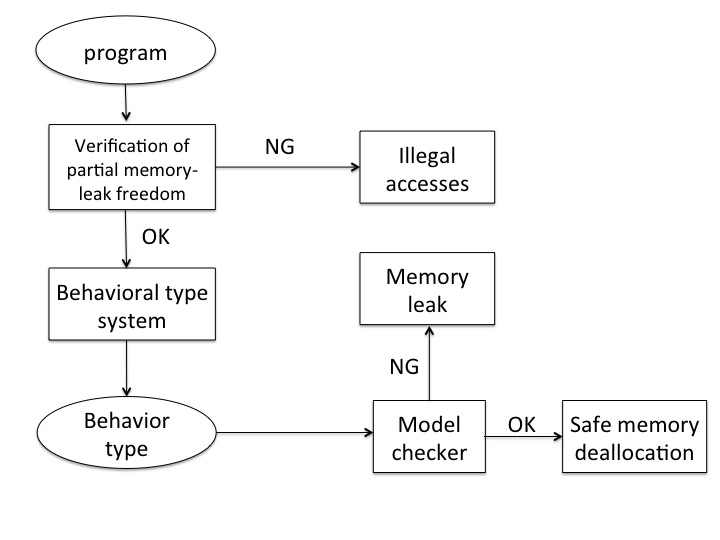
\includegraphics[width=10cm]{overview.jpg}
\caption{Overview of the algorithm}
\label{fig:ov}
\end{figure}

As represented in Figure~\ref{fig:ov}, a program is first checked by \textbf{SK} type system; if the properties about no double frees or illegal read/write operations to a deallocated memory cell is guaranteed, then it returns ``OK'' and the program is passed to our behavior type system, and it returns ``NG'' otherwise; our behavior type system will produce a behavioral type, and this behavioral type is passed to a model checker like \texttt{SPIN} or \texttt{CPAChecker} to verify whether it is consumed upper bound of memory cells.

Hence, by using our type system with \textbf{SK} type system, we can verify memory-leak freedom even for nonterminating programs.

The rest of this paper is structured as follows. Section 2 introduces a simple imperative language, as well as its syntax and operational semantics. Section 3 introduces the behavioral type system, which describes how to guarantee memory-leak freedom for non-terminating programs. Section 4 proposes an inference algorithm, and talks about syntax directed typing rules. Section 5 describes current status and future work.

\section{Language}
This section introduces a sublanguage of Suenaga and Kobayashi~\cite{DBLP:conf/aplas/SuenagaK09} with primitives for memory allocation/deallocation. The values in our paper are only pointers. \\
The syntax of language is as follows.

\paragraph{Notation.} we write $\vec{x}$ for a sequence $x_{1} \dots x_{n}$, and $x_{1} \dots x_{n}$ are pairwise-distinct; $f\{x\rightarrow v \}$ denotes a function $f'$ such that $f'(y) = v$ if $x = y$, otherwise $f'(y) = f(y)$ and $y \in dom(f)$; $[v/x]s$ denotes that substituting $v$ for $x$ in $s$.

  \begin{flalign*}
  s \ (\mathit{statements}) &::=  \SKIP \tB s_{1};s_{2} \tB *x \leftarrow y \tB \Free \Cirx\\
  &\tB \LET x = \MALLOC \IN s \tB \LET x = \NULL \IN s  \\
  &\tB \LET x = y \; \IN s \tB   \LET x = *y \; \IN s \\
  &\tB \IFNULL(x) \; \THEN s_{1}\; \ELSE s_{2} \tB f(\vec{x}) \\
  d \ (\mathit{definition}) &::= f(x_{1},\dots,x_{n}) = s
  \end{flalign*}

The command $\SKIP$ does nothing. The command $s_{1};s_{2}$ is executed as a sequence, first executing $s_{1}$ and then $s_{2}$. The command $*x \leftarrow y$ updates the content of the memory cell which is pointed by pointer $x$ with value $y$. The command $\Free \Cirx$ deallocates the memory cell which is pointed to by a pointer $x$. Command $\LET x = e \; \IN s$ first evaluates the expression $e$, binds $x$ to the result, and then executes statement $s$. The command $\LET x = \Malloc() \; \IN s$ first allocates a memory cell, binds $x$ to the pointer to the cell then executes the statement $s$. The command $\LET x = \NULL  \IN s$ binds $x$ to a null pointer and then executes $s$. The command $\LET x = y \; \IN s$ binds $x$ to $y$ and then executes statement $s$. The command $\LET x = *y \; \IN s$ binds $x$ to the contents of the cell pointered to by $y$ and executes statement $s$. The command $\IFNULL(x) \; \THEN s_{1} \; \ELSE s_{2}$ executes the statement $s_{1}$ if the pointer $x$ is a null pointer, executes statement $s_{2}$ otherwise. The command $f(\vec{x})$ is a function call $f$ with arguments $\vec{x}$; we assume that the sequence $\vec{x}$ is pairwise-distinct. $d$ denotes the definition of function $f(\vec{x})$ which has a body of statement $s$.

\subsection{Operational Semantics}
%% Because we want to estimate the number of available memory cells at every operation step, we extend the triple $\langle H\coma R\coma s \rangle$ that is represented as run-time state in previous type system to a quadruple $\langle H\coma R\coma s\coma n \rangle$ in our paper. The introduced notation $n$ denotes the number of available memory cells, a nature number. When executing the operation $\Malloc$, the number of available memory cells will decrease 1, which is denoted as ($n - 1$); when executing the operation $\Free$, the number of available memory cells will increase 1, which is denoted as ($n + 1$). The notation $H$, which models heap memory, is a mapping from finite subset of $\mathcal{H}$ to $\mathcal{H}$ $\cup$ \{$null$\}, where $\mathcal{H}$ represents the set of \emph{heap addresses}. $R$, which models registers, is a mapping from finite set of variables to $\mathcal{H}$ $\cup$ \{$null$\}.

%% Transition rules are listed in Figure 3. In these rules, $f\{x\to v\}$ is defined as a function $f'$ such that $f'(y) = v$ if $x = y$, otherwise $f'(y) = f(y)$ and $y \in dom(f)$. There are three rules about $\mathbf{NullEx}$ which denotes accessing a null pointer, three rules about $\mathbf{Error}$ for accessing a deallocated memory cell, and one rule about $\mathbf{Error}$ which denotes allocating a memory cell when there is no memory space.
%\begin{figure}[h]
% Skip Command
Runtime state is represented by $\langle H, R, s, n \rangle$, where $H$ is a mapping from finite subset of $\mathcal{H}$ to $\mathcal{H}$ $\cup$ \{$null$\}, in which $\mathcal{H}$ represents the set of \emph{heap addresses}, intuitively, the $H$ models a heap memory; $R$, which models registers, is a mapping from finite set of variables to $\mathcal{H}$ $\cup$ \{$null$\}.

Operational semantics are defined by the relations: $\rightarrow_{D}, \xlongrightarrow{\Malloc}_{D}, and \xlongrightarrow{\Free}_{D} $, in which $\xlongrightarrow{\Malloc}_{D}, and \xlongrightarrow{\Free}_{D} $ denote performing a allocation and deallocation operation respectively, and $\rightarrow_{D}$ expresses that performing an internal action like $\SKIP$ or assignment.

$$
    \frac{n \in \mathbb{N}}
            {\langle H\coma R\coma  \SKIP;s , n \rangle
              \longrightarrow_{D}
                \langle H\coma R\coma   s , n \rangle }
     \Rtab \mbox{(E-Skip)}
$$
% Assignment
$$
     \frac{R(x) \in dom(H), n \in \mathbb{N}}
           {\langle H\coma R\coma  *x \leftarrow y , n \rangle
             \longrightarrow_{D}
             \langle H \Lfc R(x) \rightarrow R(y) \Rfc \coma R \coma   \SKIP , n  \rangle }
     \Rtab \mbox{(E-Assign)}
$$
% Free Command
$$
     \frac{R(x) \in dom(H) , n \in \mathbb{N}}
          {\langle H\coma R\coma  \FREE , n \rangle
            \xlongrightarrow{\Free}_{D}
            \langle H\backslash \Lfc R(x) \Rfc \coma R \coma   \SKIP , n+1  \rangle }
     \Rtab \mbox{(E-Free)}
$$
% Let Null Command
$$
     \frac{x' \notin dom(R)}
           {\langle H\coma R\coma  \LET x = \NULL \IN s , n \rangle
             \longrightarrow_{D}
             \langle H\coma R\Lfc x' \rightarrow \NULL \Rfc \coma   \Lb x'/x \Rb s , n  \rangle }
     \Rtab \mbox{(E-LetNull)}
$$
% Let Eq Command
$$
     \frac{x' \notin dom(R)}
            {\langle H\coma R\coma \LET x = y \; \IN s , n \rangle
              \longrightarrow_{D}
              \langle H\coma R\Lfc x' \rightarrow R(y) \Rfc \coma   \Lb x'/x \Rb s , n  \rangle }
\Rtab \mbox{(E-LetEq)}
$$
% Reference Command
$$
     \frac{x' \notin dom(R)}
            {\langle H\coma R\coma  \LET x = *y \; \IN s , n \rangle
              \longrightarrow_{D}
              \langle H\coma R\Lfc x' \rightarrow H(R(y)) \Rfc \coma   \Lb x'/x \Rb s , n  \rangle }
     \Rtab \mbox{(E-LetDref)}
$$
% Malloc (allocate) Command
$$
     \frac{h \notin dom(H)}
            {\langle H\coma R\coma  \LET x = \Malloc() \; \IN s , n \rangle
              \xlongrightarrow{\Malloc}_{D}
              \langle H \Lfc h \rightarrow v\Rfc \coma R\Lfc x' \rightarrow h \Rfc \coma   \Lb x'/x \Rb s , n-1  \rangle }
\Rtab \mbox{(E-Malloc)}
$$
% IFNULL T
$$
    \frac{R(x) = \NULL}
           {\langle H \coma R \coma \IFNULL\Cirx   \THEN   s_{1} \ELSE\  s_{2} \coma  n \rangle
           \longrightarrow_{D}
           \langle H\coma R\coma s_{1} \coma n \rangle}
    \Rtab \mbox{(E-IfNullT)}
$$
% IFNULL F
$$
    \frac{R(x) \neq \NULL}
           {\langle H \coma R \coma \IFNULL\Cirx \THEN  s_{1} \ELSE  s_{2} \coma  n \rangle
           \longrightarrow_{D}
           \langle H\coma R\coma s_{2} \coma  n, \rangle}
    \Rtab \mbox{(E-IfNullF)}
$$
% Function Call
$$
     \frac{f(\vec{y}) = s \in D}
            { \langle H\coma R\coma  f(\vec{x}) , n \rangle
               \longrightarrow_{D}
               \langle H\coma R\coma  \Lb \vec{x}/\vec{y} \Rb s , n \rangle}
      \Rtab \mbox{(E-Call)}
$$
% Error : access the null memory cell
$$
      \frac{R(x) = null}
            {\langle H\coma R\coma  *x \leftarrow y , n \rangle
              \longrightarrow_{D}
             \bf NullEx }
      \Rtab \mbox{(E-AssignNullError)}
$$
% ERROR : access the null memory cell
$$
      \frac{R(y) = null}
             {\langle H\coma R\coma  x = *y, n \rangle
               \longrightarrow_{D}
              \bf NullEx }
             \Rtab \mbox{(E-DrefNullError)}
$$
$$
     \frac{R(x) =  null }
           {\langle H\coma R\coma  \FREE , n \rangle
             \xlongrightarrow{\Free}_{D} \bf NullEx  }
      \Rtab \mbox{(E-FreeNullError)}
$$
% ERROR :
$$
     \frac{R(x) \notin dom(H) \cup \Lfc null \Rfc}
           {\langle H\coma R\coma   *x \leftarrow y,  n \rangle
             \longrightarrow_{D}
           \bf  Error }
    \Rtab \mbox{(E-AssignError)}
$$
% ERROR
$$
      \frac{R(y) \notin dom(H) \cup \Lfc null \Rfc}
           {\langle H\coma R\coma  \LET x  = *y \; \IN s, n \rangle
              \longrightarrow_{D}
                \bf  Error }
      \Rtab \mbox{(E-DrefError)}
$$
%
$$
      \frac{R(x) \notin dom(H) \cup \Lfc null \Rfc}
            {\langle H\coma R\coma  \FREE , n \rangle
              \xlongrightarrow{\Free}_{D}
              \bf Error }
     \Rtab \mbox{(E-FreeError)}
$$
 % ERROR: no enough space
$$
      \langle H\coma R\coma \LET x = \Malloc() \ \IN s ,  0  \rangle
      \xlongrightarrow{\Malloc}_{D}
      \mathbf{Error}
      \Rtab \mbox{(E-MallocError)}
$$
$$
     \mathbf{Figure \; 3.} \;\;  \mbox{ Operational Semantics}
$$
%
%\caption{Operational Semantics.}
%\label{example:os}
     %\end{figure}
\begin{myDef}
memory leaks: if a program consumes unbounded number of memory cells.\\
memory-leak \ freedom: $\exists n \in \mathbb{N}$ s.t. $\langle \emptyset, \emptyset, s, n \rangle \nrightarrow^{*}Error$
\label{df:ml}
\end{myDef}

\section{Type System}

\subsection{Syntax of Types}
     \begin{eqnarray*}
       P (\mathit{behavioral\ types})::=&& {\bf 0} \tB P_{1};P_{2} \tB P_{1}+P_{2} \tB \Malloc\\
       &&\tB \Free \tB \alpha \tB \mu\alpha.P \\
       \sigma (\mathit{function\ types})::=&& (\tau_{1},\dots, \tau_{n}) P
     \end{eqnarray*}

The type $\bf 0$ abstracts the behavior of $\SKIP$ and means "does nothing". $P_{1};P_{2}$ is for sequential execution. $P_{1} + P_{2}$ is abstracted as conditional. $\Malloc$ is the behavior of a statement that allocates a memory cell exactly once. $\Free$ is for deallocating memory cell exactly once. $\mu \alpha. P$ is a recursive type. For example, the behavior of  the body of function $h$ in Figure 2 is abstracted as $\mu \alpha. \Malloc;\Malloc;\Free;\Free;\alpha$. $\alpha$ is a type variable and bounded to the recursive constructor $\mu \alpha$.

The only value in our paper is reference, and its type is $\mathbf{Ref}$.

The function type is described as $(\tau_{1}, \dots, \tau_{n})P$, which means a function receives some pointers as arguments and its body is abstracted as a behavioral type $P$.

% Semantics of Behavioral Types %
\subsection{Semantics of Behavioral Types}
The semantics of behavioral type are given by labeled transition system, and listed as follows:
    $$
        \mathbf{0};P \rightarrow P
    $$
    $$
          \Malloc \xlongrightarrow{\Malloc} 0
    $$
    $$
           \Free \xlongrightarrow{\Free} 0
    $$
    $$
          \mu \alpha.P \rightarrow  [\mu \alpha . P/\alpha]  P
    $$
   $$
          P_{1} + P_{2} \longrightarrow P_{1}
   $$
   $$
          P_{1} + P_{2} \longrightarrow P_{2}
   $$
   $$
           \frac{P_{1} \xlongrightarrow{\alpha} P_{1}' }
                 {P_{1};P_{2} \xlongrightarrow{\alpha} P_{1}';P_{2}}
   $$
The notation $\rightarrow$ denotes that a behavioral type can be reduced by the internal action. Notation $\xlongrightarrow{\alpha}$ means that a behavioral type can be reduced by executing $\alpha$ actions, and the $\alpha$ here is $\{\Malloc, \Free\}$.

% Type Judgments
\subsection{Typing Rules}
The type judgment of our type system is given by the form $\Theta ; \Gamma \vdash s : P$, where $\Theta$ is a mapping from function variables to function types, $\Gamma$ is a type environment that denotes a mapping from variables to value types.
It reads ``the behavior of $s$ is abstracted as $P$ under $\Theta$ and $\Gamma$ environments''. We design the type system so that this type judgment implies the property: when $s$ executes $\Malloc$(resp.$\Free$), then $P$ is equivalent to $\Malloc;P'$(resp.$\Free;P'$) for a type $P'$ such that $\Theta; \Gamma \vdash s': P'$, where $s'$ is the continuation of $s$. This property guarantees the behavioral type soundly abstracts the upper bound of the consumed memory cells.

Typing rules are presented in Figure~\ref{fig:typingrules}. In the rule for assignment, the behavior of  $*x \leftarrow y$ is $\bf 0$. The rule for $\Free$ represents that the behavior of $\Free \Cirx$ is $\Free$. The rule T-Malloc represents that $\LET x = \MALLOC \; \IN s$ has the behavior $\Malloc;P$, where $P$ is the behavior of statement $s$. The rule for function call represents that function $f$ has the behavior $P$ which is the behavior of the body of this function .

In the rule for subtyping, $P_{1} \le P_{2}$ represents that $P_{1}$ is the subtype of $P_{2}$ and  means that: \\
(1) if $P_{1} \xlongrightarrow{\alpha}  P_{1}'$ then $\exists P_{2}' $ s.t. $P_{2} \overset{\text{$\alpha$}}{\Longrightarrow} P_{2}'$ and $ P_{1}' \le P_{2}' $\\
(2) if $P_{1} \rightarrow P_{1}'$ then $\exists P_{2}'$ s.t. $P_{2} \rightarrow^{*} P_{2}'$ and  $P_{1}' \le P_{2}'$\\
where $\overset{\text{$\alpha$}}{\Longrightarrow}$ means that: $\rightarrow^{*} \xlongrightarrow{\alpha} \rightarrow^{*}$.

At the end of $s$, memory leak freedom is guaranteed by $OK_{n}(P)$ ,where $P$ is the behavior of $s$. $OK_{n}(P)$ is defined as Definition~\ref{df:okn} in which $\sharp_{malloc}(\alpha)$ and $\sharp_{free}(\alpha)$ are functions to count the number of $\Malloc$ and $\Free$ actions in $\alpha$ respectively. This definition, intuitively, means at every running step the number of allocated memory cells will never go out of memory scope.
\begin{myDef}
  $OK_{n}(P) \iff \forall P',\; P \xlongrightarrow{\alpha}^{*}P'$ then $\sharp_{malloc}(\alpha)-\sharp_{free}(\alpha)\le n$.
\label{df:okn}
\end{myDef}

\begin{figure}
\begin{boxedminipage}{12cm}
  \scriptsize

% Skip type
$$
         \Theta ; \Gamma \vdash \SKIP : \mathbf{0}
      \Rtab \mbox{(T-Skip)}
$$
% Sequence type
$$
      \frac{\Theta ; \Gamma \vdash s_{1} : P_{1} \Rtab \Theta ; \Gamma \vdash s_{2} : P_{2}}
          {\Theta ; \Gamma \vdash s_{1} ; s_{2} : P_{1};P_{2} }
     \Rtab \mbox{(T-Seq)}
$$
% Assignment type
$$
     \frac{\Theta ; \Gamma \vdash y  \Rtab \Theta ; \Gamma \vdash x }
          {\Theta ; \Gamma \vdash *x \leftarrow y : \mathbf{0} }
     \Rtab \mbox{(T-Assign)}
$$
% Free(deallocate) type
$$
     \frac{\Theta ; \Gamma \vdash x  }
           {\Theta ; \Gamma \vdash \Free(x) : \Free}
     \Rtab \mbox{(T-Free)}
$$
% Malloc type
$$
     \frac{\Theta ; \Gamma,x \vdash s : P}
           {\Theta ; \Gamma \vdash \LET x = \MALLOC \; \IN s  : \Malloc;P}
           \Rtab \mbox{(T-Malloc)}
$$
% Let eq type
$$
     \frac{\Theta ; \Gamma \vdash y   \Rtab \Theta ; \Gamma , x  \vdash s : P}
           {\Theta ; \Gamma \vdash \LET x = y \; \IN s : P}
     \Rtab \mbox{(T-LetEq)}
$$
% Dereference type
$$
     \frac{\Theta ; \Gamma \vdash y  \Rtab \Theta ; \Gamma , x  \vdash s : P}
           {\Theta ; \Gamma \vdash \LET x = *y \; \IN s : P}
     \Rtab \mbox{(T-LetDref)}
$$
% Let NULL type
$$
     \frac{\Theta ; \Gamma, x  \vdash s : P}
           {\Theta ; \Gamma \vdash \LET x = \mathbf{null} \; \IN s : P}
     \Rtab \mbox{(T-LetNull)}
$$
% Subtyping
$$
     \frac{\Theta ; \Gamma \vdash s : P_{1} \Rtab P_{1} \le P_{2}}
            {\Theta ; \Gamma \vdash s : P_{2}}
     \Rtab \mbox{(T-Sub)}
$$
 % ifnull s then s type
$$
     \frac{\Theta ; \Gamma \vdash x    \ \ \ \  \Theta ; \Gamma \vdash s_{1} : P \ \ \ \ \Theta ; \Gamma \vdash s_{1} : P}
           {\Theta ; \Gamma \vdash \IFNULL(x) \; \THEN s_{1}\; \ELSE s_{2} : P}
     \Rtab \mbox{(T-IfNull)}
$$
% Function call type
$$ \frac{ \Theta(f) = P}
{\Theta; \Gamma, \vec{x} : \vec{\tau} \vdash f(\vec{x}) : P}
\Rtab \mbox{(T-Call)} $$
% Program
$$\frac{\vdash D : \Theta \;\;\;\; \Theta; \emptyset\vdash s : P \Rtab OK_{n}(P)}
{\vdash (D, s)}
\Rtab \mbox{(T-Program)} $$
\end{boxedminipage}
\caption{Typing Rules}
\label{fig:typingrules}
\end{figure}

\subsection{Type Soundness}
This subsection describes some theorems and lemmas for type safety.
\begin{theorem}\label{thm1}
If $\vdash (D, s)$ then $(D, s)$ does not lead to $memory\;leak$.\\
Memory leak freedom: $\exists n \in \mathbb{N}$ s.t.
$\langle \emptyset, \emptyset, s, n \rangle \nrightarrow^{*}Error$
\end{theorem}
\noindent
This theorem says that a well typed program guarantees memory leak freedom.
% Lemma Preservation %
\begin{lemma}[Preservation $\mathbf{I}$]%\label{preser}
If $OK_{n}(P)$, $\Theta; \Gamma \vdash s : P$ and $\langle H,R,s, n \rangle
\xlongrightarrow{\alpha}\langle H',R',s', n'
\rangle$, then $\exists P'$ s.t. \\
(1) $ \Theta; \Gamma \vdash s' : P' $ \\
(2) $ P \overset{\text{$\alpha$}}{\Longrightarrow} P'$\\
(3) $ OK_{n'}(P') $
\end{lemma}
\begin{lemma}[Preservation $\mathbf{II}$]%\label{preser}
If $OK_{n}(P)$, $\Theta ; \Gamma \vdash s : P$ and $\langle H,R,s,n \rangle
\rightarrow \langle H',R',s', n'
\rangle$, then $\exists P'$ s.t. \\
(1) $\Theta; \Gamma \vdash s' : P'$\\
(2) $ P \rightarrow^{*} P'  $\\
(3) $OK_{n'}(P')$
\end{lemma}
\begin{lemma}%\label{error}
 The partial correctness is guaranteed $\vdash \langle H,R,s \rangle$ , so that if $\vdash \langle H,R,s,n \rangle$, then $\vdash \langle H',R',s',n' \rangle \nrightarrow Error$
\end{lemma}
\section{Type Inference Algorithm}
This section describes how to construct syntax directed typing rules according to the typing rules of above section, and it provides an algorithm which inputs statements and returns a pair containing constraints and behavior types.
\subsection{Constraints Generation}
By syntax directed typing rules, the type inference algorithm has been designed as in Figure~\ref{fig:tyin}.

Function $PT_{v}(x) = (C,\emptyset)$ denotes that it receives a pointer variable $x$ and outputs a pair consisting of constraints set $C$ and an empty set. $PT_{\Theta}(s) = (C, P)$ is a mapping from statements to a pair --  constraints set $C$ and behavioral types $P$, where $\Theta$ is mapping from function names to function types. $PT(\langle D,s \rangle) = (C, P)$ denotes that it receives a program and produces a pair $(C, P)$. $\alpha_{i}$ and $\beta$ are fresh type variables.

\begin{figure}
\begin{boxedminipage}{8cm}
  \scriptsize
\begin{nospaceflalign*}
   PT_{\Theta}(f) &  =  &\\
  & \ \  \LET  \alpha = \Theta(f) & \\
  & \ \ \IN   (C = \{\alpha \le \beta \}, \beta) &
\end{nospaceflalign*}
\begin{nospaceflalign*}
   PT_{\Theta}(\SKIP) &  =  (\emptyset, 0)&
\end{nospaceflalign*}
\begin{nospaceflalign*}
   PT_{\Theta}(s_{1}&;s_{2})  =  &\\
   & \ \ \ \LET (C_{1}, P_{1}) = PT_{\Theta}(s_{1}) & \\
   &\ \ \ \ \ \ \  \ (C_{2}, P_{2}) = PT_{\Theta}(s_{2}) & \\
   & \ \ \ \IN   (C_{1} \cup C_{2}\cup \{P_{1}; P_{2} \le \beta \}, \beta) &
\end{nospaceflalign*}
\begin{nospaceflalign*}
   PT_{\Theta}(*x& \leftarrow y)   =  &\\
  & \ \ \LET (C_{1}, \emptyset) = PT_{v}(*x) & \\
  & \ \ \ \ \ \ (C_{2}, \emptyset) = PT_{v}(y) & \\
  &\ \  \IN    (C_{1} \cup C_{2},  0) &
\end{nospaceflalign*}
\begin{nospaceflalign*}
   PT_{\Theta}(\Free(x)) &  = (\emptyset, \Free)  &
\end{nospaceflalign*}
\begin{nospaceflalign*}
   PT_{\Theta}(\LET &x = \Malloc() \  \IN s)  =  &\\
   &\LET (C_{1}, P_{1}) = PT_{v}(s) & \\
   &\IN  (C_{1} \cup \{P_{1} \le \beta \} ,  \Malloc; \beta) &
\end{nospaceflalign*}
\begin{nospaceflalign*}
   PT_{\Theta}(\LET &x = y \  \IN s )  =  &\\
   &  \LET (C_{1}, \emptyset) = PT_{v}(y) & \\
   & \ \ \ \ \ (C_{2}, P_{1}) = PT_{\Theta}(s) & \\
   &  \IN   (C_{1} \cup C_{2}\cup \{P_{1} \le \beta \},  \beta) &
\end{nospaceflalign*}
\begin{nospaceflalign*}
   PT_{\Theta}(\LET &x = *y \  \IN s )  =  &\\
   & \LET  (C_{1}, \emptyset) = PT_{v}(y) & \\
   &\ \ \ \ \ \ (C_{2}, P_{1}) = PT_{\Theta}(s) & \\
   & \IN   (C_{1} \cup C_{2}\cup \{P_{1} \le \beta \},  \beta) &
\end{nospaceflalign*}
\begin{nospaceflalign*}
   PT_{\Theta}(&\IFNULL(x) \  \THEN  s_{1} \  \ELSE \ s_{2} )  =  &\\
   & \ \ \ \ \ \LET  (C_{1}, P_{1}) = PT_{\Theta}(s_{1}) & \\
   &\ \ \ \ \  \ \ \ \ \ (C_{2}, P_{2}) = PT_{\Theta}(s_{2}) & \\
   &\ \ \ \ \  \ \ \ \ \ (C_{3}, \emptyset) = PT_{v}(x) & \\
   & \ \ \ \ \ \ \IN   (C_{1} \cup C_{2}\cup C_{3}\cup \{P_{1} \le \beta, P_{2} \le \beta \},  \beta) &
\end{nospaceflalign*}
\begin{nospaceflalign*}
   PT(\langle D, s \rangle&)   =  &\\
   &\LET  \Theta = \{ f_{1}:\alpha_{1}, \dots, f_{n}:\alpha_{n}  \} &\\
   & \ \ \ \ \  where \ \{ f_{1},\dots, f_{n} \} = dom(D) \ and \ \alpha_{1}, \dots, \alpha_{n} \  are \ fresh  & \\
   & \IN    \LET  (C_{i}, P_{i}) = PT_{\Theta}(D(f_{i})) \  for \  each \ i & \\
   & \IN    \LET  C_{i}^{'} = \{ \alpha_{i} \le P_{i} \} \ for \  each \ i & \\
   & \IN    \LET  (C, P) = PT_{\Theta}(s)  & \\
   & \IN   (C_{i} \cup C_{i}^{'} ) \cup C \cup  \{OK(P)\},  P) &
\end{nospaceflalign*}
\end{boxedminipage}
\caption{Type Inference Algorithm}
\label{fig:tyin}
\end{figure}

\subsection{Constraints Reduction}
Given a closed process $P$, $PT(P)$ produces a triple. The subtype constraints on behavior types of the form $\alpha \ge A$, and constraints of the form $OK_{n}(P)$. Thus, we obtain the following constraints:\\
$$
\{ \alpha_{1} \ge A_{1}, \dots, \alpha_{n} \ge  A_{n}, OK_{n}(B)\}
$$
Here, we can assume that $\alpha_{1}, \dots, \alpha_{n}$ are pairwise-distinct, since $\alpha \ge A_{1}$ and $\alpha \ge A_{2}$ can be replaced with $\alpha \ge A_{1}+A_{2}$ by lemma 3.8 in paper~\cite{DBLP:journals/lmcs/KobayashiSW06}. we can also assume that $\{ \alpha_{1}, \dots, \alpha_{n} \}$ contains all the type variables in the constraints, since otherwise we can always add the tautology $\alpha \ge \alpha$. Each subtype constraints $\alpha \ge A$ can be replaced by $\alpha \ge \mu \alpha. A$, by lemma 3.8(4)~\cite{DBLP:journals/lmcs/KobayashiSW06} ( substituting $\alpha$ for $B$ in this lemma). Therefore the above constraints can be further reduced to $OK_{n}([\vec{A} \backslash \vec{\alpha}])$. Here, $A'_{1}, \dots, A'_{n}$ are the least solutions for the subtype constraints.

\section{Preliminary Experiment}

\section{Related Work}

\section{Conclusion}
We have described a type-based approach to safe memory deallocation for non-terminating programs. The approach is based on the idea of decomposing safe memory memory deallocation into partial correctness, which is verified by previous type system, and behavioral correctness. We designed a behavioral type system in our paper for verification of behavioral correctness. Currently, we are looking for a model checker to estimate an upper bound of consumption given a behavioral type and planning to implement a verifier and conduct experiment to see whether our approach is feasible.

\bibliographystyle{IEEEtran}
\bibliography{tan}

\newpage
\appendix
\section*{Appendix}
\subsection*{1. Proof for Lemma Preservation}

By induction on the derivation of evaluation rules.\\

\noindent Case: $\langle H, R, \FREE, n \rangle \xlongrightarrow{\Free} \langle H', R', \SKIP, n + 1 \rangle $. \\

From the assumption, we have known that: \textcircled{1} $OK_{n}(P)$, and \textcircled{2} $\Theta; \Gamma \vdash \Free\Cirx:P$.

By the inversion lemma on \textcircled{2}, we have: \textcircled{3} $\Free \le P$.

From the definition of subtyping, \textcircled{3} and rule $\Free \xlongrightarrow{\Free} 0$, we get:
\begin{center}
$\exists P''$ s.t. \textcircled{4} $P \overset{\text{$\Free$}}{\Longrightarrow} P''$,  and \textcircled{5} $0 \le P''$
\end{center}

We need to prove that there exists $P'$ and $\Gamma'$ such that:
\begin{center}
\textcircled{6} $\Theta; \Gamma' \vdash \SKIP: P'$,  and \textcircled{7} $P \overset{\text{$\Free$}}{\Longrightarrow} P'$
\end{center}

Take $P''$ as $P'$. Then \textcircled{7} holds. By the typing rule T-Skip and \textcircled{5}, we get:
$$
   \frac{\Theta; \Gamma' \vdash \SKIP : 0 \ \ \ \  0 \le P''}
   {\Theta; \Gamma' \vdash \SKIP : P''}
   \Rtab \mbox{(T-Sub)}
$$

Therefore, \textcircled{6} holds. \\

\noindent Case: $\langle H, R, \LET x = \MALLOC \IN s_{1}, n \rangle \xlongrightarrow{\Malloc} \langle H', R', [x'/x]s_{1}, n - 1  \rangle $.\\

From the assumption, we already have \textcircled{1}$\Theta; \Gamma \vdash \LET x = \MALLOC \IN s_{1} : P$,

and \textcircled{2} $OK_{n}(P)$.

By the inversion lemma and \textcircled{1}, we have \textcircled{3} $\Malloc;P_{1} \le P$, and \textcircled{4} $\Theta; \Gamma \vdash s_{1} : P_{1}$

We need to find $P'$ and $\Gamma'$ such that \textcircled{5} $\Theta; \Gamma' \vdash s_{1} : P'$, and \textcircled{6}$P \overset{\text{$\Malloc$}}{\Longrightarrow} P'$

Because of the following derivation:
$$
  \frac{ \Malloc \xlongrightarrow{\Malloc} 0}
  {\Malloc;P_{1} \xlongrightarrow{\Malloc} 0;P_{1}}
$$

and $0;P_{1} \Rightarrow P_{1}$. Therefore $\Malloc;P_{1} \xlongrightarrow{\Malloc} P_{1}$.

By the definition of subtyping and $\Malloc;P_{1} \xlongrightarrow{\Malloc} P_{1}$, we have that:
\begin{center}
$\exists P''$ s.t. \textcircled{7} $P \overset{\text{$\Malloc$}}{\Longrightarrow} P''$, and \textcircled{8} $P_{1} \le P''$
 \end{center}

Taking $P''$ as $P'$, then \textcircled{6} holds.

And by using subtyping rule T-Sub with premises \textcircled{4} and \textcircled{8}
$$
    \frac{\Gamma \vdash s_{1} : P_{1} \ \ \ \ P_{1} \le P''}
     {\Gamma \vdash s_{1} : P''}
     \Rtab \mbox{(T-Sub)}
$$

Therefore we prove that $\Gamma \vdash s_{1} : P'$, \textcircled{5} holds.\\

\noindent Case: $\langle H, R, \SKIP;s_{1}, n \rangle \rightarrow \langle H', R', s_{1}, n \rangle $. \\

From the assumption, we have
\begin{center}
\textcircled{1} $\Theta; \Gamma \vdash \SKIP;s_{1} : P$, and \textcircled{2} $OK_{n}(P)$
\end{center}

By the inversion lemma on \textcircled{1}, we have
\begin{center}
\textcircled{3} $\Theta; \Gamma \vdash s_{1} : P_{1}$, and \textcircled{4} $0;P_{1} \le P $
\end{center}

We need to prove that there exists $P'$ and $\Gamma'$ such that
\begin{center}
\textcircled{5} $\Theta; \Gamma' \vdash s_{1} : P'$, and \textcircled{6} $P \rightarrow^{*} P'$
\end{center}

By the definition of subtyping and $0;P_{1} \rightarrow P_{1}$, then we get that $\exists P''$
\begin{center}
 \textcircled{7} $P \rightarrow^{*} P''$, and \textcircled{8} $P_{1} \le P''$
\end{center}

Taking $P''$ as  $P'$, we get $P \rightarrow^{*} P'$

And by using rule T-Sub with premises $\Gamma \vdash s_{1} : P_{1}$ and $P_{1} \le P''$, then we have 
$$
    \frac{\Theta; \Gamma \vdash s_{1} : P_{1} \  \  P_{1} \le P''}
    {\Gamma \vdash s_{1} : P''}
    \Rtab \mbox{(T-Sub)}
$$

Therefore, we prove that $\Gamma \vdash s_{1} : P'$ \\

\noindent Case: $\langle H, R, *x \leftarrow y , n \rangle \rightarrow  \langle H', R', \SKIP, n  \rangle $. \\

From the assumption, we already have
\begin{center}
\textcircled{1} $\Theta; \Gamma \vdash *x \leftarrow y : P$, and \textcircled{2} $OK_{n}(P)$
\end{center}

From the inversion lemma on \textcircled{1}, we have \textcircled{3} $0 \le P$.

We need to find $P'$ and $\Gamma'$ such that
\begin{center}
 \textcircled{4} $\Theta; \Gamma' \vdash \SKIP: P'$, and \textcircled{5} $P \rightarrow^{*} P'$
\end{center}

Taking $P$ as $P'$, then \textcircled{5} holds.

And because of the following derivation:
$$
  \frac{\Theta; \Gamma' \vdash \SKIP: 0 \ \ \ 0 \le P}
   {\Theta;\Gamma' \vdash \SKIP : P}
  \Rtab \mbox{(T-Sub)}
$$
therefore \textcircled{4} holds. \\

\noindent Case: $\langle H, R, \LET x = y\  \IN s_{1} , n \rangle \rightarrow  \langle H', R', [x'/x]s_{1}, n  \rangle $. \\

From assumption, we have 
\begin{center}
\textcircled{1} $\Theta; \Gamma \vdash \LET x = y\  \IN \  s_{1} : P$, and \textcircled{2} $OK_{n}(P)$.
\end{center}

From the inversion lemma and \textcircled{1}, we have 
\begin{center}
\textcircled{3} $\Theta; \Gamma \vdash s_{1} : P_{1}$, and $P_{1} \le P$.
\end{center}

We need to find $P'$ and $\Gamma'$ such that:
\begin{align}
  &\Theta; \Gamma' \vdash s_{1} : P' \ \ and& \label{eq5.4.1}\\
  &P \xlongrightarrow{\tau}^{*} P'& \label{eq5.4.2}
\end{align}

Taking P as P'. Therefore \eqref{eq5.4.2} holds, because of the definition of $\rightarrow^{*}$.

And because of the following derivation, \eqref{5.4.1} holds.
$$
  \frac{\Theta; \Gamma' \vdash s_{1} : P_{1} \ \ \ P_{1} \le P}
  {\Theta; \Gamma' \vdash s_{1} : P}
  \Rtab \mbox{(T-Sub)}
$$

\noindent Case: $\langle H, R, \LET x = \NULL \  \IN \  s_{1}, n \rangle \rightarrow \langle H', R', [x'/x]s_{1}, n \rangle $\\

From the assumption, we know that
\begin{center}
\textcircled{1}$\Theta; \Gamma \vdash \LET x = \NULL \  \IN \ s_{1} : P$, and \textcircled{2} $OK_{n}(P)$.
\end{center}

By inversion lemma on \eqref{eqa.1}, we get:
\begin{center}
$\Theta; \Gamma \vdash s_{1} : P_{1}$, and $ P_{1} \le P$.
\end{center}

We need to prove that there exists $P'$ and $\Gamma'$ such that
\begin{center}
$\Theta; \Gamma' \vdash s_{1} : P'$, and $P \rightarrow^{*} P'$.
\end{center}

Taking P as P'. Because of the following derivation, the \eqref{eqa.5} holds.
$$
  \frac{\Theta; \Gamma' \vdash s_{1} : P_{1} \ \ \ \ P_{1} \le P}
  {\Theta; \Gamma' \vdash s_{1} : P}
  \Rtab \mbox{(T-Sub)}
$$

And because of the definition of $\xlongrightarrow{\tau}^{*}$, the \eqref{eqa.6} holds. \\

\noindent Case: $\langle H, R, \LET x = *y \  \IN \  s_{1}, n \rangle \rightarrow \langle H', R', [x'/x]s_{1}, n \rangle $\\

From the assumption, we know that
\begin{center}
$\Theta; \Gamma \vdash \LET x = *y \  \IN \  s_{1} : P$, and $OK_{n}(P)$.
\end{center}

By the inversion lemma on \eqref{eqb.1}, we get:
\begin{center}
$\Theta; \Gamma \vdash s_{1} : P_{1}$, and $P_{1} \le P$.
\end{center}

We need to prove there exists $P'$ and $\Gamma'$ such that:
\begin{center}
$\Theta; \Gamma' \vdash s_{1} : P'$, and $P \rightarrow^{*} P'$.
\end{center}

Taking P as P'. Because of  following derivation, the \eqref{eqb.5} holds.
$$
   \frac{\Theta; \Gamma' \vdash s_{1} : P_{1} \ \ \ P_{1} \le P}
   {\Theta; \Gamma' \vdash s_{1} : P}
   \Rtab \mbox{(T-Sub)}
$$

And because of the definition of $\xlongrightarrow{\tau}^{*}$, \eqref{eqb.6} holds. \\

\noindent Case $\langle H, R, \IFNULL \Cirx \  \THEN s_{1} \  \ELSE \  s_{2}, n \rangle \rightarrow \langle H', R',s_{1}, n \rangle $\\

From the assumption, we have that:
\begin{center}
$\Theta; \Gamma \vdash \IFNULL \Cirx \  \THEN \  s_{1} \ \ELSE \ s_{2} : P$, and $OK_{n}(P)$.
\end{center}

By the inversion leamma on \eqref{eqc.1}, we get:
\begin{center}
$\Theta; \Gamma \vdash s_{1} : P_{1}$, and $ p_{1} \le P'$.
\end{center}

We need to prove that there exists $P'$ and $\Gamma'$ such that:
\begin{center}
 $\Theta; \Gamma' \vdash s_{1} : P_{1}$, and $P \rightarrow^{*} P'$.
\end{center}

Taking P as P'. Because of the following derivation, \eqref{eqc.5} holds.
$$
  \frac{\Theta; \Gamma' \vdash s_{1} : P_{1} \ \ \ \ P_{1} \le P}
  {\Theta; \Gamma' \vdash s_{1} : P}
  \Rtab \mbox{(T-Sub)}
$$

And by the definition of $\xlongrightarrow{\tau}^{*}$, \eqref{eqc.6} holds. \\

\noindent Case: $\langle H, R, f(x) , n \rangle \rightarrow  \langle H', R', [x'/x]s_{1}, n  \rangle $ where the body of function $f(x)$ is $s_{1}$. we can see $f(x)$ and $s_{1}$ as $s$ and $s'$ respectively. \\

From the assumption, we already have
\begin{center}
$\Gamma \vdash f(x) : P$, and $OK_{n}(P)$.
\end{center}

By the inversion lemma and \eqref{eq6.1}, we have
\begin{center}
$P_{1} \le P$, and $\Gamma \vdash s_{1} : P_{1}$.
\end{center}

From the definition of subtyping and $P_{1} \xlongrightarrow{0} P_{1}$, we get $\exists P''$ s.t.
\begin{center}
$P \xlongrightarrow{0} P''$, and $P_{1} \le P''$.
\end{center}

Taking the $P''$ to be $P'$, then we get $P \xlongrightarrow{0} P'$.\\
And by using the subtyping rule with premises \eqref{eq6.4} and  \eqref{eq6.6}, we have
$$
\frac{\Gamma \vdash s_{1} : P_{1} \ \ \ \ P_{1} \le P'}{\Gamma \vdash s_{1} : P'}
$$

Therefore we prove that $\Gamma \vdash s' : P'$ where $s'$ is the command $s_{1}$.

\noindent Finally to prove $OK_{n'}P'$ that is, $\sharp_{m}(P')-\sharp_{f}(P') \le n'$. And  proceed by case analysis.\\

\noindent Case $P =  \SKIP;P'$\\

According to rule E-Skip, we should prove  $\sharp_{m}(P')-\sharp_{f}(P') \le n'$ where $n'$ is $n$.

Because we have
\begin{eqnarray*}
  OK_{n}(P)  & & =  OK_{n}(\SKIP;P')\\
  & & \Rightarrow \sharp_{m}(\SKIP;P') - \sharp_{f}(\SKIP;P') \le n \\
  & & \Rightarrow \sharp_{m}(P') - \sharp_{f}(P') \le n \
\end{eqnarray*}
Then it is proved. \\

\noindent Case $P = \Malloc;P'$ \\

Here according to rule E-Malloc, we know the $n'$ is $n-1$.

Therefore we should prove $\sharp_{m}(P') - \sharp_{f}(P') \le n-1$
\begin{eqnarray*}
  OK_{n}(P)&& =  OK_{n}(\Malloc;P')\\
  &&\Rightarrow \sharp_{m}(\Malloc;P') - \sharp_{f}(\Malloc;P') \le n \\
  &&\Rightarrow  \sharp_{m}(P') + 1 - \sharp_{f}(P') \le n\\
  &&\Rightarrow  \sharp_{m}(P')  - \sharp_{f}(P') \le n-1\\
\end{eqnarray*}

Then it is proved.\\

\noindent Case $P = \Free;P'$ \\

According to rule E-Free, we should prove $\sharp_{m}(P') - \sharp_{f}(P') \le n+1$.

\begin{eqnarray*}
  OK_{n}(P)  & & =  OK_{n}(\Free;P')\\
  & &\Rightarrow  \sharp_{m}(\Free;P') - \sharp_{f}(\Free;P') \le n \\
  & & \Rightarrow \sharp_{m}(P')  - \sharp_{f}(P') - 1  \le n\\
  & & \Rightarrow \sharp_{m}(P')  - \sharp_{f}(P') \le n+1\\
\end{eqnarray*}

Then it is proved. \\

\noindent Case $P = P_{1};P_{2}$\\

To prove it by contradiction.

Suppose that $OK_{n'}(P_{1}';P_{2})$ does not hold. Then we have 
$P_{1};P_{2} \xlongrightarrow{\alpha} P_{1}';P_{2} \xlongrightarrow{\exists \sigma} Q$, $s.t.$ $\sharp_{m}(\sigma) - \sharp_{f}(\sigma) > n'$\\

From the premise $OK_{n}(P) = OK_{n}(P_{1};P_{2})$, we get 
\setcounter{equation}{0}
\begin{align}
  &  \sharp_{m}(\alpha \cdot \sigma) - \sharp_{f}(\alpha \cdot \sigma) \le n \label{eqok1.1}
\end{align}

From \eqref{eqok1.1}, we get
\begin{align}
\sharp_{m}(\alpha) + \sharp_{m}(\sigma) - \sharp_{f}(\alpha) - \sharp_{f}(\sigma) \  \label{eqok1.2}
\end{align}
and with
$$
   n'=\left\{
   \begin{aligned}
     n + 1, && \alpha = \Free \\
     n - 1,  && \alpha = \Malloc  \\
     n ,      && otherwise
   \end{aligned}
   \right.
$$
Therefore, we get \\
$n' + \sharp_{m}(\alpha) - \sharp_{f}(\alpha) < \sharp_{m}(\alpha) + \sharp_{m}(\sigma) - \sharp_{f}(\alpha) - \sharp_{f}(\sigma) \le n $ \\
When $\alpha = \Free$, we get that $n + 1 - 1 < n$\\
When $\alpha = \Malloc$, we get that $ n - 1 + 1 < n $ \\
When $ \alpha = other$,  we  get that $ n < n $ \\
 All of the three cases are equal to $n$. Therefore we get the contradiction.

\subsection*{2. Syntax Directed Typing Rules}
Typing rules showed in Figure  are not immediately suitable for type inference. The reason is that the subtyping rule can be applied to any kind of term. This means that, any kind of term $s$ can be applied by either subtyping rule or the other rule whose conclusion matches the shape of the $s$ \cite{plain:book1}.

In order to yield a type inference algorithm, we should do something with the subtyping rule. The method is to merge the subtyping rule with the other rules by introducing a set $C$ of constraints, where $C$ consists of subtype constraints on behavioral types of the form $P_{1}\le P_{2}$ and $OK_{n}(P)$.

Syntax directed typing rules are listed in Figure 

$$
     \frac{ C = \emptyset}
           {\Theta; \Gamma; C \vdash \SKIP : \mathbf{0}}
      \Rtab \mbox{(ST-Skip)}
$$
$$
      \frac{\Theta;\Gamma ; C_{1} \vdash s_{1} : P_{1} \Rtab \Theta; \Gamma ; C_{2} \vdash s_{2} : P_{2} \Rtab C = C_{1}\cup C_{2} \cup \{ P_{1};P_{2} \le P\}}
      {\Theta;\Gamma; C \vdash s_{1};s_{2} : P}
      \Rtab \mbox{(ST-Seq)}
$$
$$
      \frac{\Theta;\Gamma;C_{1} \vdash y \Rtab \Theta;\Gamma; C_{2} \vdash x : \mathbf{Ref} \Rtab C = C_{1}\cup C_{2}}
      {\Theta;\Gamma; C \vdash *x \leftarrow y : \mathbf{0}}
      \Rtab \mbox{(ST-Assign)}
$$
$$
      \frac{C = \emptyset}
      {\Gamma ; C \vdash \Free() : \Free}
     \Rtab \mbox{(ST-Free)}
$$
$$
     \frac{\Theta;\Gamma, x ; C_{1} \vdash s : P_{1} \Rtab C = C_{1} \cup\{P_{1}\le P\}}
     {\Theta;\Gamma; C \vdash \LET x = \Malloc() \; \IN s : \Malloc ; P}
     \Rtab \mbox{(ST-Malloc)}
$$
$$
     \frac{\Theta;\Gamma; C_{1} \vdash y \Rtab \Theta;\Gamma, x ; C_{2} \vdash s : P_{1} \Rtab C = C_{1}\cup C_{2} \cup \{P_{1} \le P \}}
     {\Theta;\Gamma ; C \vdash \LET x = y \;  \IN s : P}
     \Rtab \mbox{(ST-LetEq)}
$$
$$
     \frac{\Theta;\Gamma ; C_{1} \vdash y: \mathbf{Ref} \Rtab \Theta;\Gamma, x ; C_{2} \vdash s : P_{1} \Rtab C = C_{1}\cup C_{2}\cup\{P_{1} \le P\}}
     {\Theta;\Gamma ; C \vdash \LET x = *y \; \IN s : P}
     \Rtab \mbox{(ST-LetDref)}
$$
$$
     \frac{\Theta;\Gamma; C_{1} \vdash x \Rtab \Theta;\Gamma; C_{2} \vdash s_{1} : P_{1} \Rtab \Theta;\Gamma; C_{3} \vdash s_{2} : P_{2}  \Rtab  C = C_{1} \cup C_{2} \cup C_{3} \{P_{1}\le P, P_{2}\le P \}}
     {\Theta;\Gamma; C \vdash \IFNULL\Cirx \THEN s_{1} \ELSE s_{2} : P }
    \; \;  \mbox{(ST-IfNull)}
$$
$$
     \frac{\Theta(f) = P_{1} \Rtab C = P_{1} \le P}
     {\Gamma,\vec{x}:\vec{\tau} \vdash f(\vec{x}) : P }
     \Rtab \mbox{(ST-Call)}
$$
$$
     \frac{\Theta \vdash D : \Theta \Rtab \Theta ; \emptyset ; C_{1} \vdash s : P \Rtab C = C_{1}\cup\{OK_{n}(P)\}}
     {C \vdash (D , s) }
     \Rtab \mbox{(ST-Program)}
$$
$$
    \mathbf{Figure \; 5.} \;\; \mbox{Syntax Directed Typing Rules}
$$

\end{document}
